\documentclass{article}
\usepackage[utf8]{inputenc}
\usepackage[backend=biber]{biblatex}
\usepackage{amssymb}
\usepackage{amsmath}
\usepackage{dsfont}
\addbibresource{bib.bib}
\setlength{\parindent}{0em}
\bibliography{bib}
\setlength{\parskip}{6pt}
\usepackage[margin=1.0in]{geometry}
\usepackage{graphicx}
\usepackage{caption}
\usepackage{subcaption}
\usepackage{wrapfig}
\usepackage{url}

\title{Intro to deep learning with PyTorch}
\author{Miguel A. Saavedra-Ruiz}
\date{May 2020}
\linespread{1.0}

\nocite{*}


\begin{document}

\maketitle

\section*{Convolutional Neural Networks}

Convolutional Neural Networks (CNNs) are a variation of neural networks with the ability to efficiently operate over images. CNNs can look at images as a whole and learn to identify spatial patterns such as prominent colors and shapes, or whether a texture is fuzzy or smooth and so on. The shapes and colors that define any image and any object in an image are often called \textbf{features} Fig. \ref{fig:f1}.

An example of a feature would be what do we look at to distinguish a cat and a dog. These characteristics might be the shape of the eyes, the size, and how they move are just a couple of examples of visual features. 

\begin{figure}[ht]
    \centering
    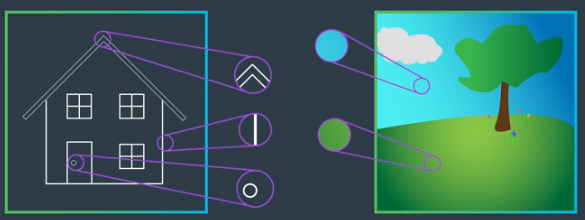
\includegraphics[width=0.45\textwidth,height=0.45\textheight,keepaspectratio]{images/features.png}
    \captionsetup{justification=centering}
    \caption{Features in an image}
    \label{fig:f1}
\end{figure}





\printbibliography

\end{document}
